\documentclass[aspectratio=169,11pt]{beamer}

\usepackage[T1]{fontenc}
\usepackage{lmodern}
\usepackage{microtype}
\usepackage{amsmath,amssymb}
\usepackage{tikz}
\usepackage{pgfplots}
\pgfplotsset{compat=1.18}

\usetheme{zibtalk}
% figures/styles.tex -- shared TikZ styles and helpers for all figures.
%
% Conventions (so the pictures stay easy to edit):
%   * x = time, 1 unit = 1 time unit; y = rows.  Everything sits on a 0.5 grid.
%   * A schedule is a list of \job / \refam bars with plain numbers:
%       \job[row]{colour}{start}{end}{label}     processing that makes progress
%       \refam[row]{colour}{start}{end}          re-familiarization (no progress)
%     [row] is the y-coordinate of the bar's lower edge (default 0).
%   * \timeaxis[row]{from}{to} draws a time axis with integer ticks.
%   * Inside \foreach, wrap \job / \refam in braces: \foreach \s in {..} { \job.. }
%   * Scale a whole figure with the [x=..cm,y=..cm] option of its tikzpicture.

\usetikzlibrary{arrows.meta,patterns,decorations.pathreplacing}

% job colours
\definecolor{jobA}{RGB}{0,64,150}
\definecolor{jobB}{RGB}{215,110,0}
\definecolor{jobC}{RGB}{0,135,105}
\definecolor{jobD}{RGB}{130,60,150}
\colorlet{other}{black!45}

\newcommand{\barh}{0.6}% bar height in y-units (\renewcommand inside a figure to change)

\tikzset{
  >={Stealth[length=5pt]},
  lbl/.style      = {font=\footnotesize},
  leg/.style      = {lbl, anchor=west, text height=1.5ex, text depth=0.3ex},% legend text
  bar/.style      = {draw=#1!85!black, fill=#1!30, line width=0.6pt},
  hatched/.style  = {draw=#1!85!black, line width=0.6pt, preaction={fill=#1!8},
                     pattern=north east lines, pattern color=#1!75},
  axis/.style     = {->, line width=0.6pt, black!70},
  tick/.style     = {line width=0.6pt, black!70},
  guide/.style    = {densely dashed, line width=0.5pt, black!45},
  brace/.style    = {decorate, decoration={brace, amplitude=4pt}, line width=0.6pt, black!70},
  bracedown/.style= {decorate, decoration={brace, amplitude=4pt, mirror}, line width=0.6pt, black!70},
  rowlabel/.style = {lbl, anchor=east, xshift=-5pt},
  endlabel/.style = {lbl, anchor=west, xshift=6pt},
}

% \job[row]{colour}{start}{end}{label}
\newcommand{\job}[5][0]{%
  \draw[bar=#2] (#3,#1) rectangle node[lbl]{#5} (#4,#1+\barh);}
% \refam[row]{colour}{start}{end}
\newcommand{\refam}[4][0]{%
  \draw[hatched=#2] (#3,#1) rectangle (#4,#1+\barh);}
% \timeaxis[row]{from}{to}: axis with integer ticks, just below the given row
\newcommand{\timeaxis}[3][0]{%
  \draw[axis] (#2,#1-0.15) -- (#3+0.6,#1-0.15) node[right,lbl]{time};
  \foreach \t in {#2,...,#3}
    \draw[tick] (\t,#1-0.15) -- ++(0,-0.1) node[below,lbl]{$\t$};}
% \timearrow[row]{from}{to}: axis without ticks
\newcommand{\timearrow}[3][0]{%
  \draw[axis] (#2,#1-0.15) -- (#3+0.6,#1-0.15) node[right,lbl]{time};}
% \barlegend{x}{y}: legend "progress / re-familiarization" with lower-left corner (x,y)
\newcommand{\barlegend}[2]{%
  \draw[bar=jobA]     (#1,#2)     rectangle ++(0.5,0.3);
  \node[leg] at (#1+0.6,#2+0.15) {progress};
  \draw[hatched=jobA] (#1+2.5,#2) rectangle ++(0.5,0.3);
  \node[leg] at (#1+3.1,#2+0.15) {re-familiarization};}
   % shared TikZ styles; each picture is one file in figures/

% --- talk metadata (short title / author appear in the footer) -----------
\title[Lossy Preemption]{Non-Clairvoyant Scheduling with Lossy Preemption}
\author[Maximilian Schicker]{Maximilian Schicker\affil{1,2}}
\email{schicker@zib.de}
\coauthors{Sven J\"ager\affil{2}, Max Klimm\affil{2} and Phillip Warode\affil{3}}
\institute{\affil{1}\,Zuse Institute Berlin \quad
  \affil{2}\,Technische Universit\"at Berlin \quad
  \affil{3}\,Humboldt-Universit\"at zu Berlin}
\date{ITCS 2027}

% --- notation -------------------------------------------------------------
% \src{key} / \src[note]{key}: small grey citation, clickable (jumps to the References frame)
\newcommand{\src}[2][]{{\footnotesize\color{ztgray}%
  \if\relax\detokenize{#1}\relax\cite{#2}\else\cite[#1]{#2}\fi}}
\setbeamertemplate{bibliography item}[text]
\setbeamercolor{bibliography item}{fg=zibblue}
\setbeamercolor{bibliography entry author}{fg=black}
\setbeamercolor{bibliography entry title}{fg=zibblue}
\setbeamercolor{bibliography entry location}{fg=ztgray}
\setbeamercolor{bibliography entry note}{fg=ztgray}
\newcommand{\doi}[1]{\href{https://doi.org/#1}{doi:\,\detokenize{#1}}}
\newcommand{\norm}[1]{\lVert #1 \rVert}
\newcommand{\Alg}{\mathrm{Alg}}
\newcommand{\Opt}{\mathrm{Opt}}
\newcommand{\WRR}{\mathrm{WRR}}

\begin{document}

\begin{frame}[plain]
  \titlepage
\end{frame}

% =========================================================================
\section[Setting]{Non-Clairvoyant Scheduling}

\begin{frame}{Focus on one task, or multitask?}
  \begin{itemize}
    \item One machine, jobs $j = 1,\dots,n$ available at time $0$,
          weights $w_j$, processing times $p_j$
    \item Goal: minimize the total weighted completion time $\sum_j w_j C_j$
    \item Known $p_j$: run jobs in order of $p_j / w_j$ --- optimal,
          and \alert{no preemption needed} \src{smith56}
  \end{itemize}
  \vfill
  \centering
  % Clairvoyant scheduling: shortest job first vs. longest job first.
% Unit weights, p = (1, 2, 4).
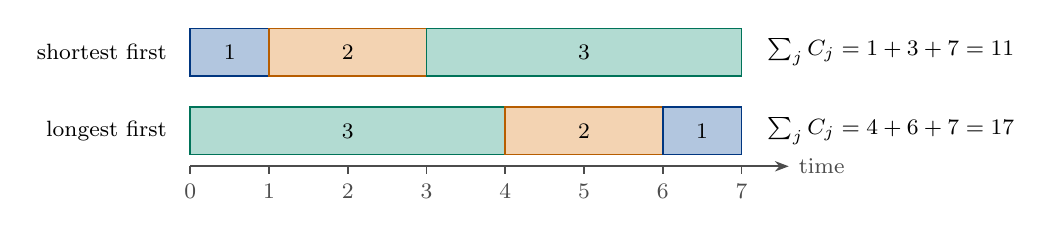
\begin{tikzpicture}[x=1cm,y=1cm]
  % --- row y=1: shortest processing time first -------------------------
  \node[rowlabel] at (0,1.3) {shortest first};
  \job[1]{jobA}{0}{1}{$1$}
  \job[1]{jobB}{1}{3}{$2$}
  \job[1]{jobC}{3}{7}{$3$}
  \node[endlabel] at (7,1.3) {$\sum_j C_j = 1+3+7 = 11$};
  % --- row y=0: longest processing time first --------------------------
  \node[rowlabel] at (0,0.3) {longest first};
  \job{jobC}{0}{4}{$3$}
  \job{jobB}{4}{6}{$2$}
  \job{jobA}{6}{7}{$1$}
  \node[endlabel] at (7,0.3) {$\sum_j C_j = 4+6+7 = 17$};
  \timeaxis{0}{7}
\end{tikzpicture}

\end{frame}

\begin{frame}{More general: the weighted $k$-norm}
  \begin{itemize}
    \item We minimize the \textbf{weighted $k$-norm} of completion times, for any $k \ge 1$:
      \[ \norm{C}_{k,w} = \Bigl(\,\sum_{j=1}^{n} w_j\, C_j^{\,k}\Bigr)^{1/k} \]
  \end{itemize}
  \centering
  % The weighted k-norm interpolates between the sum (k = 1) and the maximum (k -> infinity).
% Marks at x = 0, 4, 10; formulas below, meaning below that.
\begin{tikzpicture}[x=1cm,y=1cm]
  \draw[axis] (-0.5,0) -- (11,0) node[right,lbl]{$k$};
  % --- marks: position / label above / formula / meaning -------------------
  \foreach \x/\k/\f/\m in {
      0/{k=1}/{\sum_j w_j C_j}/{average},
      4/{k=2}/{\bigl(\sum_j w_j C_j^{2}\bigr)^{1/2}}/{},
      10/{k\to\infty}/{\max_j C_j}/{worst case (makespan)}} {
    \draw[tick, line width=1pt] (\x,0.15) -- (\x,-0.15);
    \node[lbl, above] at (\x,0.2)  {$\k$};
    \node[lbl]        at (\x,-0.7) {$\f$};
    \node[lbl, jobA]  at (\x,-1.3) {\m};
  }
  % --- what changes along the axis ------------------------------------------
  \draw[->, alertred, line width=0.7pt] (1.5,0.9) -- node[above,lbl]{late completions weigh more and more} (8.5,0.9);
\end{tikzpicture}

  \vfill
  \begin{itemize}
    \item \textbf{Why?} The sum only rewards a good average: single jobs may finish very late.
          The maximum ignores everything but the last job.
    \item The $k$-norm \alert{balances average performance and fairness}
          \src{bp10}\,\src{mv22}
  \end{itemize}
\end{frame}

\begin{frame}{What if durations are unknown?}
  \begin{itemize}
    \item \textbf{Non-clairvoyant:} $p_j$ is revealed only when job $j$ completes
    \item Committing to a job is risky: it may turn out to be very long
  \end{itemize}
  \vfill
  \centering
  % Non-clairvoyant and non-preemptive: the adversary makes the first job long.
% One long job (length M, drawn 6 units wide) and six short jobs (0.25 wide).
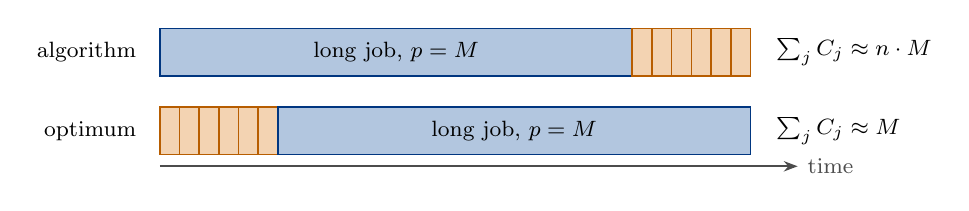
\begin{tikzpicture}[x=1cm,y=1cm]
  % --- row y=1: the algorithm commits to a job that turns out to be long --
  \node[rowlabel] at (0,1.3) {algorithm};
  \job[1]{jobA}{0}{6}{long job, $p = M$}
  \foreach \s in {6,6.25,...,7.25} { \job[1]{jobB}{\s}{\s+0.25}{} }
  \node[endlabel] at (7.5,1.3) {$\sum_j C_j \approx n\cdot M$};
  % --- row y=0: the optimum runs the short jobs first --------------------
  \node[rowlabel] at (0,0.3) {optimum};
  \foreach \s in {0,0.25,...,1.25} { \job{jobB}{\s}{\s+0.25}{} }
  \job{jobA}{1.5}{7.5}{long job, $p = M$}
  \node[endlabel] at (7.5,0.3) {$\sum_j C_j \approx M$};
  \timearrow{0}{7.5}
\end{tikzpicture}

  \vfill
  \begin{itemize}
    \item \alert{No non-preemptive algorithm has a constant competitive ratio:}
          it is $\Omega(n)$, even with randomization \src[Prop.~2.1]{jssw25}
    \item So an algorithm must preempt --- but what does a preemption cost?
  \end{itemize}
\end{frame}

\begin{frame}{Preemption: two classical models}
  \begin{columns}[t]
    \begin{column}{0.47\textwidth}
      \begin{block}{Lossless preemption}
        Switching between jobs is free.
        \begin{itemize}
          \item Round-robin is $2$-competitive for $\sum_j C_j$ \src{mpt94}
          \item $(k+1)^{1/k}$ for the $k$-norm \src{mv22}
        \end{itemize}
      \end{block}
    \end{column}
    \begin{column}{0.47\textwidth}
      \begin{block}{Kill-and-restart}
        An interrupted job starts from scratch.
        \begin{itemize}
          \item $b$-scaling: $1 + 3\sqrt{3} \approx 6.20$
          \item randomized: $\approx 3.03$ \src{jssw25}
        \end{itemize}
      \end{block}
    \end{column}
  \end{columns}
  \vfill
  \begin{center}
    In practice, returning to an interrupted task costs time ---\\
    \alert{less than starting over, but more the further you had come.}
  \end{center}
\end{frame}

% =========================================================================
\section[Model]{Lossy Preemption}

\begin{frame}{The lossy preemption model}
  \begin{columns}[c]
    \begin{column}{0.42\textwidth}
      \begin{itemize}
        \item \textbf{Recall factor} $\gamma \in [0,1]$
        \item A job with progress $Y$ is interrupted
        \item When it resumes, the first $(1-\gamma)\,Y$ time units are
              \alert{re-familiarization}: no new progress
        \item After processing for $\tau$ time units:
              \[ Y' = \max\{\,Y,\ \gamma Y + \tau\,\} \]
        \item \alert{Progress never decreases:} an interval shorter than
              $(1-\gamma)\,Y$ is wasted, $Y' = Y$
      \end{itemize}
    \end{column}
    \begin{column}{0.56\textwidth}
      \centering
      % Lossy preemption: progress of one job over time.
% The job runs during [0,2], is interrupted, and resumes during [3.5,6.5].
% At the interruption its progress is Y = 2; the plot shows gamma = 1/2:
%   re-familiarization lasts (1-gamma)*Y = 1, i.e. [3.5,4.5].
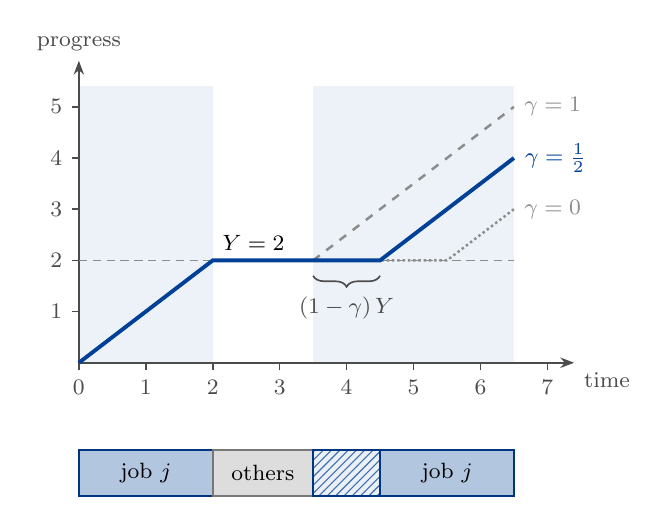
\begin{tikzpicture}[x=0.85cm,y=0.65cm]
  \renewcommand{\barh}{0.9}
  % --- processing intervals (light background) ---------------------------
  \fill[jobA!7] (0,0)   rectangle (2,5.4);
  \fill[jobA!7] (3.5,0) rectangle (6.5,5.4);
  % --- axes ---------------------------------------------------------------
  \draw[axis] (0,0) -- (7.4,0) node[below right,lbl]{time};
  \draw[axis] (0,0) -- (0,5.9) node[above,lbl]{progress};
  \foreach \t in {0,...,7} \draw[tick] (\t,0) -- ++(0,-0.15) node[below,lbl]{$\t$};
  \foreach \y in {1,...,5} \draw[tick] (0,\y) -- ++(-0.1,0) node[left,lbl]{$\y$};
  % --- progress level at the interruption --------------------------------
  \draw[guide] (0,2) -- (6.5,2);
  \node[lbl,anchor=south west] at (2,2) {$Y = 2$};
  % --- the two classical extremes (grey) ---------------------------------
  \draw[line width=0.9pt, black!45, dashed]         (3.5,2) -- (6.5,5) node[right,lbl]{$\gamma = 1$};
  \draw[line width=0.9pt, black!45, densely dotted] (3.5,2) -- (5.5,2) -- (6.5,3) node[right,lbl]{$\gamma = 0$};
  % --- progress for gamma = 1/2 -------------------------------------------
  \draw[line width=1.4pt, jobA] (0,0) -- (2,2) -- (3.5,2) -- (4.5,2) -- (6.5,4)
    node[right,lbl]{$\gamma = \tfrac12$};
  \draw[bracedown] (3.5,1.7) -- node[below=4pt,lbl]{$(1-\gamma)\,Y$} (4.5,1.7);
  % --- the same schedule as a Gantt strip ---------------------------------
  \job[-2.6]{jobA}{0}{2}{job $j$}
  \job[-2.6]{other}{2}{3.5}{others}
  \refam[-2.6]{jobA}{3.5}{4.5}
  \job[-2.6]{jobA}{4.5}{6.5}{job $j$}
\end{tikzpicture}

    \end{column}
  \end{columns}
\end{frame}

\begin{frame}{Between kill-and-restart and lossless preemption}
  \centering
  % The same situation under three recall factors.
% Job j (p_j = 4) runs during [0,2], another job runs during [2,3], then j resumes.
% Re-familiarization takes (1-gamma)*2 time units: 0, 1, 2.
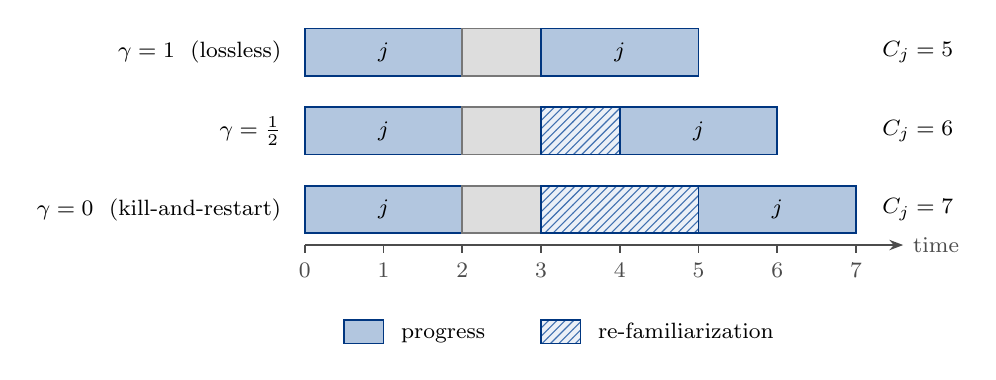
\begin{tikzpicture}[x=1cm,y=1cm]
  % --- row y=2: gamma = 1 --------------------------------------------------
  \node[rowlabel] at (0,2.3) {$\gamma = 1$ \ (lossless)};
  \job[2]{jobA}{0}{2}{$j$}
  \job[2]{other}{2}{3}{}
  \job[2]{jobA}{3}{5}{$j$}
  \node[endlabel] at (7,2.3) {$C_j = 5$};
  % --- row y=1: gamma = 1/2 ------------------------------------------------
  \node[rowlabel] at (0,1.3) {$\gamma = \tfrac12$};
  \job[1]{jobA}{0}{2}{$j$}
  \job[1]{other}{2}{3}{}
  \refam[1]{jobA}{3}{4}
  \job[1]{jobA}{4}{6}{$j$}
  \node[endlabel] at (7,1.3) {$C_j = 6$};
  % --- row y=0: gamma = 0 --------------------------------------------------
  \node[rowlabel] at (0,0.3) {$\gamma = 0$ \ (kill-and-restart)};
  \job{jobA}{0}{2}{$j$}
  \job{other}{2}{3}{}
  \refam{jobA}{3}{5}
  \job{jobA}{5}{7}{$j$}
  \node[endlabel] at (7,0.3) {$C_j = 7$};
  \timeaxis{0}{7}
  \barlegend{0.5}{-1.4}
\end{tikzpicture}

  \vfill
  \begin{itemize}
    \item $\gamma = 1$: classical preemption \qquad $\gamma = 0$: kill-and-restart
    \item The re-familiarization time grows with the progress already made
  \end{itemize}
\end{frame}

\begin{frame}{Why this model?}
  \begin{columns}[c]
    \begin{column}{0.45\textwidth}
      \begin{itemize}
        \item \textbf{One parameter} connects the two classical models
        \item Returning to a task costs more the further you had come:
              overhead \alert{proportional to the progress}
        \item Earlier overhead models do not depend on the progress:
          \begin{itemize}
            \item fixed setup time per preemption \src{lc04}\,\src{cll12}
            \item penalty in the objective \src{blss06}
          \end{itemize}
        \item Forgetting only the \emph{last probe} instead:
              same $b$-scaling schedules (next slide)
      \end{itemize}
    \end{column}
    \begin{column}{0.53\textwidth}
      \centering
      % Why this model: time lost when resuming a job, as a function of its progress Y.
%   lossy preemption: (1-gamma)*Y  -> a line through the origin with slope 1-gamma
%   gamma = 1: slope 0 (lossless),  gamma = 0: slope 1 (kill-and-restart)
%   fixed setup time: a horizontal line (independent of the progress)
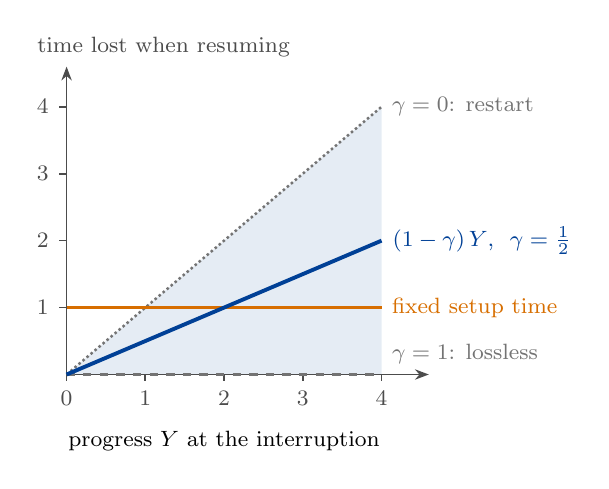
\begin{tikzpicture}[x=1cm,y=0.85cm]
  % --- all recall factors: the wedge between slope 0 and slope 1 ----------
  \fill[jobA!10] (0,0) -- (4,0) -- (4,4) -- cycle;
  % --- axes ---------------------------------------------------------------
  \draw[axis] (0,0) -- (4.6,0);
  \node[lbl] at (2,-1) {progress $Y$ at the interruption};
  \draw[axis] (0,0) -- (0,4.6) node[above right,lbl,xshift=-0.5cm]{time lost when resuming};
  \foreach \t in {0,...,4} \draw[tick] (\t,0) -- ++(0,-0.1) node[below,lbl]{$\t$};
  \foreach \y in {1,...,4} \draw[tick] (0,\y) -- ++(-0.1,0) node[left,lbl]{$\y$};
  % --- the two classical models -------------------------------------------
  \draw[line width=0.9pt, black!55, densely dotted] (0,0) -- (4,4) node[right,lbl]{$\gamma = 0$: restart};
  \draw[line width=0.9pt, black!55, dashed]         (0,0) -- (4,0) node[above right,lbl]{$\gamma = 1$: lossless};
  % --- fixed setup time (independent of progress) --------------------------
  \draw[line width=0.9pt, jobB] (0,1) -- (4,1) node[right,lbl]{fixed setup time};
  % --- lossy preemption, gamma = 1/2 ---------------------------------------
  \draw[line width=1.4pt, jobA] (0,0) -- (4,2) node[right,lbl]{$(1-\gamma)\,Y$, \ $\gamma = \tfrac12$};
\end{tikzpicture}

    \end{column}
  \end{columns}
\end{frame}

\begin{frame}{A natural variant: forgetting only the last probe}
  A job has retained progress $R$, is processed for a probe of length $\tau$, and is interrupted.
  \begin{itemize}
    \item \textbf{This talk:} the interruption shrinks \alert{all} progress:
          \ $R' = \gamma\,(R+\tau)$
    \item \textbf{Variant:} only the last probe shrinks, and only once:
          \ $R' = R + \gamma\,\tau$
  \end{itemize}
  \vfill
  \centering
  % Two forgetting models: what is retained after three probes of length tau = 4,
% each followed by an interruption (gamma = 1/2, retained progress starts at 0).
%   this talk: R' = gamma (R + tau)  -> every interruption shrinks ALL progress:
%              probe 1 keeps gamma^3 tau = 0.5, probe 2 gamma^2 tau = 1, probe 3 gamma tau = 2
%   variant:   R' = R + gamma tau    -> each probe shrinks only once: 2, 2, 2
% x = amount of work (1 unit = 1 time unit of processing); colour = probe.
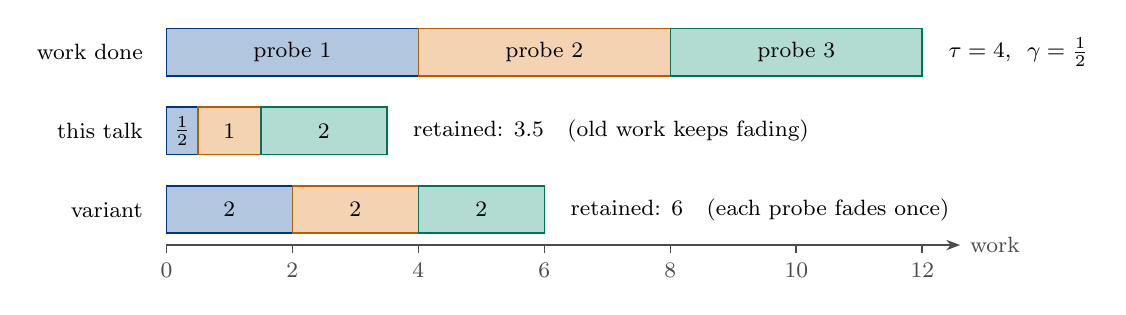
\begin{tikzpicture}[x=0.8cm,y=1cm]
  % --- row y=2: the work that was done -------------------------------------
  \node[rowlabel] at (0,2.3) {work done};
  \job[2]{jobA}{0}{4}{probe 1}
  \job[2]{jobB}{4}{8}{probe 2}
  \job[2]{jobC}{8}{12}{probe 3}
  \node[endlabel] at (12,2.3) {$\tau = 4$, \ $\gamma = \tfrac12$};
  % --- row y=1: this talk, all progress shrinks at every interruption ------
  \node[rowlabel] at (0,1.3) {this talk};
  \job[1]{jobA}{0}{0.5}{$\tfrac12$}
  \job[1]{jobB}{0.5}{1.5}{$1$}
  \job[1]{jobC}{1.5}{3.5}{$2$}
  \node[endlabel] at (3.5,1.3) {retained: $3.5$ \ \ (old work keeps fading)};
  % --- row y=0: variant, only the last probe shrinks, once -----------------
  \node[rowlabel] at (0,0.3) {variant};
  \job{jobA}{0}{2}{$2$}
  \job{jobB}{2}{4}{$2$}
  \job{jobC}{4}{6}{$2$}
  \node[endlabel] at (6,0.3) {retained: $6$ \ \ (each probe fades once)};
  % --- axis: amount of work --------------------------------------------------
  \draw[axis] (0,-0.15) -- (12.6,-0.15) node[right,lbl]{work};
  \foreach \t in {0,2,...,12}
    \draw[tick] (\t,-0.15) -- ++(0,-0.1) node[below,lbl]{$\t$};
\end{tikzpicture}

  \vfill
  \begin{itemize}
    \item Same extremes $\gamma = 0$ and $\gamma = 1$
    \item Under $b$-scaling: the same schedule as our model with recall factor
          $\gamma' = \frac{\gamma\, b}{b-1+\gamma} \ge \gamma$
  \end{itemize}
\end{frame}

\begin{frame}{Benchmark: the competitive ratio}
  \begin{itemize}
    \item \textbf{Competitive ratio} of a non-clairvoyant algorithm for the weighted $k$-norm:
      \[ \sup_{(p,w)} \; \frac{\norm{C^{\Alg}(p,w)}_{k,w}}{\norm{C^{\Opt}(p,w)}_{k,w}} \]
    \item The optimum knows all $p_j$ and never preempts
    \item Randomized algorithms: expected objective value, oblivious adversary
    \item \textbf{Question:} what is the best ratio for each norm $k$ and each recall factor $\gamma$?
  \end{itemize}
\end{frame}

\begin{frame}{Our results}
  \begin{columns}[c]
    \begin{column}{0.48\textwidth}
      \begin{itemize}
        \item \textbf{Lower bound} for every $k$ and $\gamma$\\
              ($k=1$: \ $3-\gamma$)
        \item \textbf{Upper bound} via $b$-scaling:
              \[ \bigl(2-\gamma+2\sqrt{1-\gamma}\bigr)\,(k+1)^{1/k} \]
        \item $\gamma = 1$: weighted round-robin is \alert{optimal}
        \item Randomization improves the bound
        \item $k=1$: \alert{exact} ratios of $b$-scaling
        \item Parallel machines, $\gamma = 0$:\\ ratio $4.547$ instead of $9.899$
      \end{itemize}
    \end{column}
    \begin{column}{0.5\textwidth}
      \centering
      % Lower (dashed) and upper (solid) bounds for deterministic algorithms,
% weighted k-norm of completion times, as functions of the recall factor gamma.
%   upper bound: (2 - gamma + 2 sqrt(1-gamma)) * (k+1)^(1/k)      (Theorem 2)
%   lower bound: (((2-gamma)^(k+1) - 1) / (1-gamma))^(1/k)        (Theorem 1)
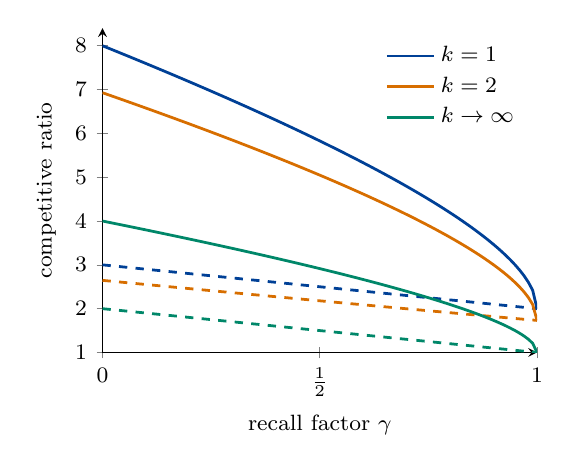
\begin{tikzpicture}
  \begin{axis}[
      width=7.1cm, height=5.7cm,
      xmin=0, xmax=1, ymin=1, ymax=8.4,
      xlabel={recall factor $\gamma$}, ylabel={competitive ratio},
      xtick={0,0.5,1}, xticklabels={$0$,$\tfrac12$,$1$},
      ytick={1,...,8},
      axis lines=left, tick label style={font=\footnotesize}, label style={font=\footnotesize},
      domain=0:1, samples=101, no markers,
      legend style={draw=none, fill=none, font=\footnotesize, at={(0.98,0.98)}, anchor=north east},
      legend cell align=left,
    ]
    % --- k = 1 ---------------------------------------------------------------
    \addplot[jobA, line width=1pt]         {2*(2-x+2*sqrt(1-x))};   \addlegendentry{$k=1$}
    \addplot[jobA, line width=1pt, dashed, forget plot] {3-x};
    % --- k = 2 ---------------------------------------------------------------
    \addplot[jobB, line width=1pt]         {sqrt(3)*(2-x+2*sqrt(1-x))}; \addlegendentry{$k=2$}
    \addplot[jobB, line width=1pt, dashed, forget plot] {sqrt(x^2-5*x+7)};
    % --- k -> infinity -------------------------------------------------------
    \addplot[jobC, line width=1pt]         {2-x+2*sqrt(1-x)};       \addlegendentry{{$k\to\infty$}}% inner braces needed: pgfplots trips over \to
    \addplot[jobC, line width=1pt, dashed, forget plot] {2-x};
  \end{axis}
\end{tikzpicture}
\\[-2pt]
      {\footnotesize\color{ztgray} solid: upper bound \quad dashed: lower bound}
    \end{column}
  \end{columns}
\end{frame}

% =========================================================================
\section[\texorpdfstring{$b$}{b}-Scaling]{The \texorpdfstring{$b$}{b}-Scaling Algorithm}

\begin{frame}{The $b$-scaling algorithm}
  \begin{itemize}
    \item Scaling factor $b > 1$, rounds $i \in \mathbb{Z}$
    \item Round $i$: process every unfinished job $j$ until its progress
          reaches $w_j\, b^{i}$ --- or until it completes
    \item Time spent on $j$ in round $i$:\quad
          $\underbrace{(1-\gamma)\,w_j b^{i-1}}_{\text{re-familiarization}}
           \;+\; \underbrace{w_j b^{i} - w_j b^{i-1}}_{\text{new progress}}$
  \end{itemize}
  \vfill
  \centering
  % b-scaling with b = 2, gamma = 1/2, unit weights, p = (1, 3, 4).
% Round i: every unfinished job is processed until its progress reaches 2^i.
% A resumed job with progress Y first needs (1-gamma)*Y = Y/2 re-familiarization.
% (The picture starts at round 0; the algorithm itself starts at round -infinity.)
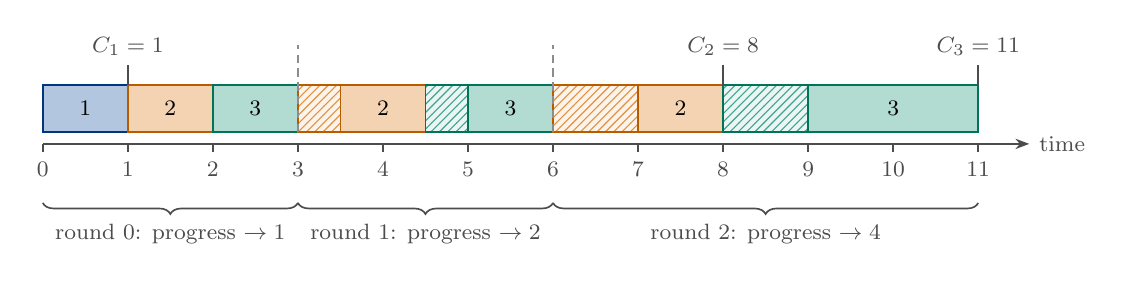
\begin{tikzpicture}[x=1.08cm,y=1cm]
  % --- round 0: target progress 1 -----------------------------------------
  \job{jobA}{0}{1}{$1$}                           % job 1 completes (p_1 = 1)
  \job{jobB}{1}{2}{$2$}
  \job{jobC}{2}{3}{$3$}
  % --- round 1: target progress 2 -----------------------------------------
  \refam{jobB}{3}{3.5}   \job{jobB}{3.5}{4.5}{$2$}
  \refam{jobC}{4.5}{5}   \job{jobC}{5}{6}{$3$}
  % --- round 2: target progress 4 -----------------------------------------
  \refam{jobB}{6}{7}     \job{jobB}{7}{8}{$2$}    % job 2 completes (p_2 = 3)
  \refam{jobC}{8}{9}     \job{jobC}{9}{11}{$3$}   % job 3 completes (p_3 = 4)
  % --- completion times ----------------------------------------------------
  \foreach \t/\j in {1/1, 8/2, 11/3}
    \draw[tick] (\t,0.6) -- (\t,0.85) node[above,lbl]{$C_{\j} = \t$};
  % --- rounds ----------------------------------------------------------------
  \foreach \t in {3,6} \draw[guide] (\t,0) -- (\t,1.1);
  \timeaxis{0}{11}
  \draw[bracedown] (0,-0.9) -- node[below=4pt,lbl]{round $0$: progress $\to 1$}  (3,-0.9);
  \draw[bracedown] (3,-0.9) -- node[below=4pt,lbl]{round $1$: progress $\to 2$}  (6,-0.9);
  \draw[bracedown] (6,-0.9) -- node[below=4pt,lbl]{round $2$: progress $\to 4$} (11,-0.9);
\end{tikzpicture}
\\[2pt]
  {\footnotesize\color{ztgray} $b = 2$, \ $\gamma = \tfrac12$, \ unit weights, \ $p = (1,3,4)$ \ (earlier rounds omitted)}
\end{frame}

\begin{frame}{Upper bound for every $k$}
  \begin{theorem}
    Deterministic $b$-scaling is $\frac{b(b-\gamma)}{b-1}\,(k+1)^{1/k}$-competitive.
    For $b = 1+\sqrt{1-\gamma}$ this is $\bigl(2-\gamma+2\sqrt{1-\gamma}\bigr)(k+1)^{1/k}$.
  \end{theorem}
  \centering
  % Geometric rounding of Smith ratios s_j = p_j / w_j (logarithmic axis).
% Thresholds b^i sit at x = 0, 3, 6, 9; each job is rounded up to the next one.
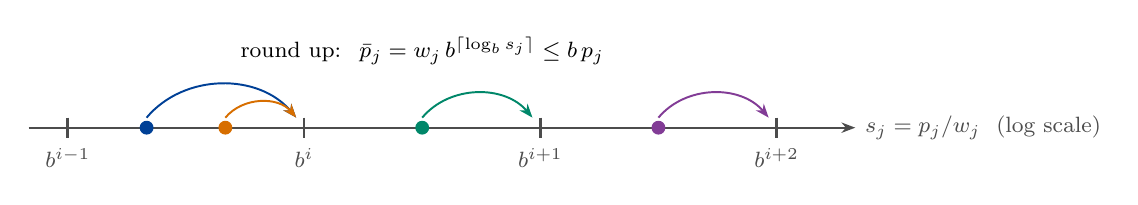
\begin{tikzpicture}[x=1cm,y=0.85cm]
  \draw[axis] (-0.5,0) -- (10,0) node[right,lbl]{$s_j = p_j/w_j$ \ (log scale)};
  % --- thresholds ----------------------------------------------------------
  \foreach \x/\l in {0/{b^{i-1}}, 3/{b^{i}}, 6/{b^{i+1}}, 9/{b^{i+2}}}
    \draw[tick, line width=1pt] (\x,0.15) -- (\x,-0.15) node[below,lbl]{$\l$};
  % --- jobs: position -> threshold it is rounded up to ---------------------
  \foreach \s/\target/\c in {1/3/jobA, 2/3/jobB, 4.5/6/jobC, 7.5/9/jobD} {
    \fill[\c] (\s,0) circle (2.5pt);
    \draw[->, \c, line width=0.7pt] (\s,0.15) to[bend left=50] (\target-0.1,0.15);
  }
  \node[lbl] at (4.5,1.15) {round up: \ $\bar p_j = w_j\, b^{\lceil \log_b s_j \rceil} \le b\, p_j$};
\end{tikzpicture}

  \vfill
  \begin{enumerate}
    \item \textbf{Inflate:} \ $p'_j = \frac{b-\gamma}{b-1}\,\bar p_j$ \ = time $b$-scaling
          spends on $j$ \ $\Rightarrow$ \ $C^{\Alg}_j(p) \le C^{\WRR}_j(p')$
    \item \textbf{Weighted round-robin} is $(k+1)^{1/k}$-competitive with lossless preemption
    \item \textbf{Compare optima:} \ $p'_j \le \frac{b-\gamma}{b-1}\, b\, p_j$
  \end{enumerate}
\end{frame}

\begin{frame}{Randomization helps}
  \begin{itemize}
    \item Random offset $\Xi \sim U[0,1]$: round $i$ has target progress $w_j\, b^{\,i+\Xi}$
    \item Random job order within each round
  \end{itemize}
  \vfill
  \centering
  % Randomized b-scaling: the thresholds b^{i+xi} are shifted by a random offset Xi.
% Deterministic thresholds at x = 0, 3, 6, 9 (grey); shifted ones at x = 1, 4, 7.
\begin{tikzpicture}[x=1cm,y=1cm]
  \draw[axis] (-0.5,0) -- (10,0) node[right,lbl]{$s_j$ \ (log scale)};
  % --- deterministic thresholds (Xi = 0) ----------------------------------
  \foreach \x/\l in {0/{b^{i-1}}, 3/{b^{i}}, 6/{b^{i+1}}, 9/{b^{i+2}}}
    \draw[tick, black!35] (\x,0.15) -- (\x,-0.15) node[below,lbl,black!45]{$\l$};
  % --- shifted thresholds (offset Xi, drawn for Xi = 1/3) ------------------
  \foreach \x/\l in {1/{b^{i-1+\Xi}}, 4/{b^{i+\Xi}}, 7/{b^{i+1+\Xi}}}
    \draw[tick, line width=1pt, alertred] (\x,0.15) -- (\x,-0.15) node[below,lbl,alertred]{$\l$};
  \draw[->, alertred, line width=0.7pt] (3,0.45) -- node[above,lbl]{$\Xi \sim U[0,1]$} (4,0.45);
  % --- a job and the threshold it is rounded up to -------------------------
  \fill[jobA] (3.25,0) circle (2.5pt);
  \draw[->, jobA, line width=0.7pt] (3.25,-0.75) -- node[below,lbl]{small rounding loss} (4,-0.75);
\end{tikzpicture}

  \vfill
  \begin{theorem}
    Randomized $b$-scaling has competitive ratio at most
    $\displaystyle \frac{b-\gamma}{b-1}\,\Bigl(\frac{b^{k}-1}{k \ln b}\Bigr)^{1/k}(k+1)^{1/k}$.
  \end{theorem}
  {\footnotesize\color{ztgray} The rounding loss $b$ is replaced by its average over the offset;
   for $k=1$ this is $\frac{b-1}{\ln b}$.}
\end{frame}

% =========================================================================
\section{Lower Bound}

\begin{frame}{A lower bound for every $k$ and $\gamma$}
  \begin{theorem}
    Every deterministic non-clairvoyant algorithm has competitive ratio at least
    \[ \Bigl(\frac{(2-\gamma)^{k+1}-1}{1-\gamma}\Bigr)^{1/k} \ \text{ for } \gamma < 1,
       \qquad (k+1)^{1/k} \ \text{ for } \gamma = 1 . \]
  \end{theorem}
  \begin{columns}[c]
    \begin{column}{0.4\textwidth}
      \begin{itemize}
        \item Many identical-looking jobs; none finishes before time $1$
        \item First interruption at time $t \ge 1$:
              all jobs are \alert{almost} done
        \item Each job still needs $(1-\gamma)\,Y_j + \delta$
      \end{itemize}
    \end{column}
    \begin{column}{0.58\textwidth}
      \centering
      % Lower bound: the adversary's move at the first interruption time t >= 1.
% Bar j shows the progress Y_j of job j at time t (drawn for gamma = 1/2):
%   lower part   = retained progress gamma*Y_j
%   hatched part = lost progress (1-gamma)*Y_j
%   red cap      = delta, since the adversary sets p_j = Y_j + delta
\begin{tikzpicture}[x=0.62cm,y=0.62cm]
  \draw[axis] (0.5,0) -- (9.4,0) node[right,lbl]{jobs};
  \draw[axis] (0.5,0) -- (0.5,3.9) node[above right,lbl,xshift=-8pt]{progress $Y_j$ at time $t$};
  % --- job / progress Y_j ----------------------------------------------------
  \foreach \j/\Y in {1/3, 2/3, 3/2, 4/2, 5/2, 6/1, 7/1, 8/1} {
    \draw[bar=jobA]     (\j,0)       rectangle (\j+0.5,0.5*\Y);   % retained
    \draw[hatched=jobA] (\j,0.5*\Y)  rectangle (\j+0.5,\Y);       % lost
    \fill[alertred]     (\j,\Y)      rectangle (\j+0.5,\Y+0.15);  % delta
  }
  % --- legend (swatch at x=6, text at x=6.8) ---------------------------------
  \fill[alertred]     (6,3.15) rectangle ++(0.5,0.15);
  \node[leg] at (6.8,3.2) {$\delta$: \ $p_j = Y_j + \delta$};
  \draw[hatched=jobA] (6,2.3)  rectangle ++(0.5,0.4);
  \node[leg] at (6.8,2.5) {lost: \ $(1-\gamma)\,Y_j$};
  \draw[bar=jobA]     (6,1.6)  rectangle ++(0.5,0.4);
  \node[leg] at (6.8,1.8) {retained: \ $\gamma\, Y_j$};
\end{tikzpicture}

    \end{column}
  \end{columns}
\end{frame}

\begin{frame}{Lower bound: the continuous limit}
  \begin{itemize}
    \item If the algorithm never interrupts after time $1$: the job it works on is very long
    \item Otherwise let $n \to \infty$: the $k$-norm becomes an $L^k$-norm of a function
    \item Chebyshev's integral inequality: the algorithm's best response is to have
          processed \alert{all jobs equally}
  \end{itemize}
  \vfill
  \begin{block}{Special cases}
    \begin{itemize}
      \item $k = 1$: \ $3 - \gamma$ \quad
            ($\gamma = 1$: $2$ \src{mpt94}, \ $\gamma = 0$: $3$ \src{jssw25})
      \item $k \to \infty$: \ $2 - \gamma$, although the makespan itself is trivial
      \item $\gamma = 1$: \ $(k+1)^{1/k}$, matched by weighted round-robin
    \end{itemize}
  \end{block}
\end{frame}

% =========================================================================
\section[Tight Bounds]{Tight Bounds and Parallel Machines}

\begin{frame}{Exact ratios for total weighted completion time}
  \begin{columns}[c]
    \begin{column}{0.48\textwidth}
      \begin{itemize}
        \item Deterministic $b$-scaling: exactly
          \[ 1 + \frac{2b^{3/2} + \gamma\,(1 - 2\sqrt{b} - b)}{b-1} \]
        \item Randomized $b$-scaling: exactly
          \[ \frac{\sqrt{b}\,(1-\gamma) + 2b - 1 - \gamma}{\sqrt{b}\,\ln b} \]
        \item Weighted mutual delays $\to$ quadratic forms $\to$ largest eigenvalue
        \item Tight instances from the eigenvectors
      \end{itemize}
    \end{column}
    \begin{column}{0.5\textwidth}
      \centering
      % Exact competitive ratios of b-scaling for total weighted completion time (k = 1),
% with the optimal scaling factor b for each recall factor gamma.
%   deterministic: 1 + (2 b^(3/2) + gamma (1 - 2 sqrt(b) - b)) / (b - 1),
%                  b = (3 - gamma + sqrt((3-gamma)^2 - 4 gamma)) / 2      (Theorem 9)
%   randomized:    (sqrt(b)(1-gamma) + 2b - 1 - gamma) / (sqrt(b) ln b),
%                  minimized numerically over b                          (Theorem 13)
\begin{tikzpicture}
  \begin{axis}[
      width=7.1cm, height=5.7cm,
      xmin=0, xmax=1, ymin=1, ymax=6.8,
      xlabel={recall factor $\gamma$}, ylabel={competitive ratio},
      xtick={0,0.5,1}, xticklabels={$0$,$\tfrac12$,$1$},
      ytick={1,...,6},
      axis lines=left, tick label style={font=\footnotesize}, label style={font=\footnotesize},
      no markers, clip=false,
      legend style={draw=none, fill=none, font=\footnotesize, at={(0.98,0.98)}, anchor=north east},
      legend cell align=left,
      declare function={
        bdet(\g)    = (3-\g+sqrt((3-\g)^2-4*\g))/2;
        rdet(\g,\b) = 1 + (2*\b^1.5 + \g*(1-2*sqrt(\b)-\b))/(\b-1);
      },
    ]
    % --- deterministic b-scaling ------------------------------------------------
    \addplot[alertred, line width=1pt, domain=0:0.999, samples=200] {rdet(x,bdet(x))};
    \addlegendentry{deterministic}
    % --- randomized b-scaling (gamma, ratio at the optimal b) -------------------
    \addplot[jobA, line width=1pt] coordinates {
      (0.00,3.0311) (0.05,2.9987) (0.10,2.9655) (0.15,2.9318) (0.20,2.8972)
      (0.25,2.8618) (0.30,2.8256) (0.35,2.7883) (0.40,2.7500) (0.45,2.7104)
      (0.50,2.6695) (0.55,2.6270) (0.60,2.5826) (0.65,2.5361) (0.70,2.4869)
      (0.75,2.4345) (0.80,2.3780) (0.85,2.3157) (0.90,2.2447) (0.95,2.1579)
      (0.98,2.0881) (0.99,2.0565) (1.00,2.0000)};
    \addlegendentry{randomized}
    % --- lower bound for deterministic algorithms -------------------------------
    \addplot[black!60, line width=1pt, dashed, domain=0:1, samples=2] {3-x};
    \addlegendentry{lower bound (det.)}
    % --- known special cases ----------------------------------------------------
    \fill[alertred] (axis cs:0,6.196) circle (2pt);
    \fill[jobA]     (axis cs:0,3.031) circle (2pt);
    \fill[black!70] (axis cs:1,2)     circle (2pt);
  \end{axis}
\end{tikzpicture}

    \end{column}
  \end{columns}
\end{frame}

\begin{frame}{Identical parallel machines}
  \centering
  % Parallel machines: random assignment, then randomized b-scaling per machine.
% Jobs are the small squares on the left; machine rows are y = 2, 1, 0.
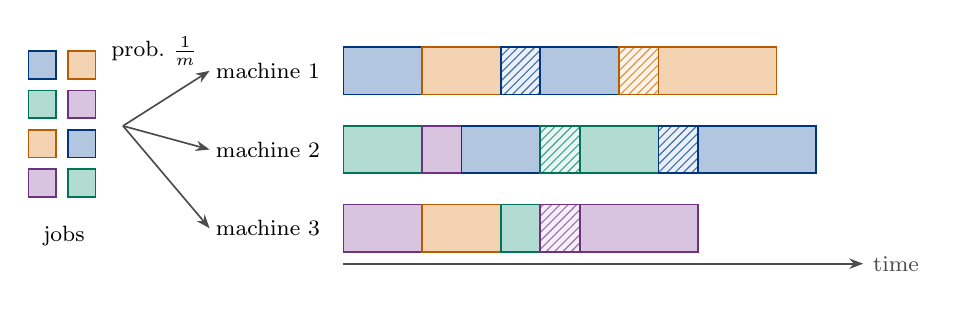
\begin{tikzpicture}[x=1cm,y=1cm]
  % --- job pool (colour = job) -------------------------------------------
  \foreach \x/\y/\c in {0/2.2/jobA, 0.5/2.2/jobB, 0/1.7/jobC, 0.5/1.7/jobD,
                        0/1.2/jobB, 0.5/1.2/jobA, 0/0.7/jobD, 0.5/0.7/jobC}
    \draw[bar=\c] (\x,\y) rectangle ++(0.35,0.35);
  \node[lbl] at (0.45,0.2) {jobs};
  % --- random assignment ---------------------------------------------------
  \foreach \y in {2.3,1.3,0.3}
    \draw[->, tick] (1.2,1.6) -- (2.3,\y);
  \node[lbl] at (1.6,2.55) {prob.\ $\tfrac1m$};
  % --- machine 1 (row y=2) -------------------------------------------------
  \node[rowlabel] at (4,2.3) {machine 1};
  \job[2]{jobA}{4}{5}{}   \job[2]{jobB}{5}{6}{}
  \refam[2]{jobA}{6}{6.5} \job[2]{jobA}{6.5}{7.5}{}
  \refam[2]{jobB}{7.5}{8} \job[2]{jobB}{8}{9.5}{}
  % --- machine 2 (row y=1) -------------------------------------------------
  \node[rowlabel] at (4,1.3) {machine 2};
  \job[1]{jobC}{4}{5}{}   \job[1]{jobD}{5}{5.5}{}  \job[1]{jobA}{5.5}{6.5}{}
  \refam[1]{jobC}{6.5}{7} \job[1]{jobC}{7}{8}{}
  \refam[1]{jobA}{8}{8.5} \job[1]{jobA}{8.5}{10}{}
  % --- machine 3 (row y=0) -------------------------------------------------
  \node[rowlabel] at (4,0.3) {machine 3};
  \job{jobD}{4}{5}{}      \job{jobB}{5}{6}{}       \job{jobC}{6}{6.5}{}
  \refam{jobD}{6.5}{7}    \job{jobD}{7}{8.5}{}
  \timearrow{4}{10}
\end{tikzpicture}

  \vfill
  \begin{itemize}
    \item Assign every job to a uniformly random machine, then run randomized
          $b$-scaling on each machine --- \alert{no migration}
    \item Competitive ratio at most $\tfrac32 \times$ the single-machine ratio
    \item $\gamma = 0$: \ $\approx 4.547$, previously $9.899$
          (deterministic, migratory, unweighted) \src{jssw25}
  \end{itemize}
\end{frame}

\begin{frame}{Summary and open problems}
  \begin{block}{Lossy preemption}
    Resuming a job with progress $Y$ costs $(1-\gamma)\,Y$ ---
    between kill-and-restart ($\gamma=0$) and lossless preemption ($\gamma=1$).
  \end{block}
  \begin{itemize}
    \item Lower and upper bounds for every $k$-norm and every $\gamma$; tight for $\gamma = 1$
    \item Exact analysis of $b$-scaling for $k=1$; non-migratory algorithm for parallel machines
  \end{itemize}
  \vfill
  \begin{exampleblock}{Open problems}
    \begin{itemize}
      \item Close the gap between lower and upper bounds for $\gamma < 1$
      \item Release dates, precedence constraints, unrelated machines
      \item Other models of forgetting: memory decay over time, recall that improves with repetition
    \end{itemize}
  \end{exampleblock}
\end{frame}

% =========================================================================
\appendix   % frames from here on do not count towards the total / progress bar
\section*{References}

\begin{frame}[allowframebreaks]{References}
  \fontsize{7.5}{9.5}\selectfont
  \begin{thebibliography}{JSSW '25}
    \bibitem[BLSS '06]{blss06}
      Y.~Bartal, S.~Leonardi, G.~Shallom, R.~Sitters.
      \newblock On the value of preemption in scheduling.
      \newblock \emph{APPROX}, 2006. \doi{10.1007/11830924_6}
    \bibitem[BP '10]{bp10}
      N.~Bansal, K.~Pruhs.
      \newblock Server scheduling to balance priorities, fairness, and average quality of service.
      \newblock \emph{SIAM J.\ Comput.}\ 39(7), 2010. \doi{10.1137/090772228}
    \bibitem[CLL '12]{cll12}
      H.-L.~Chan, T.-W.~Lam, R.~Li.
      \newblock Online flow time scheduling in the presence of preemption overhead.
      \newblock \emph{APPROX}, 2012. \doi{10.1007/978-3-642-32512-0_8}
    \bibitem[JSSW '25]{jssw25}
      S.~J\"ager, G.~Sagnol, D.~Schmidt genannt Waldschmidt, P.~Warode.
      \newblock Competitive kill-and-restart and preemptive strategies for non-clairvoyant scheduling.
      \newblock \emph{Math.\ Program.}\ 210, 2025. \doi{10.1007/s10107-024-02118-8}
    \bibitem[LC '04]{lc04}
      Z.~Liu, T.~C.~E.~Cheng.
      \newblock Minimizing total completion time subject to job release dates and preemption penalties.
      \newblock \emph{J.\ Sched.}\ 7(4), 2004. \doi{10.1023/B:JOSH.0000031424.35504.c4}
    \bibitem[MPT '94]{mpt94}
      R.~Motwani, S.~Phillips, E.~Torng.
      \newblock Nonclairvoyant scheduling.
      \newblock \emph{Theor.\ Comput.\ Sci.}\ 130(1), 1994. \doi{10.1016/0304-3975(94)90151-1}
    \bibitem[MV '22]{mv22}
      B.~Moseley, S.~Vardi.
      \newblock The efficiency-fairness balance of round robin scheduling.
      \newblock \emph{Oper.\ Res.\ Lett.}\ 50(1), 2022. \doi{10.1016/j.orl.2021.11.008}
    \bibitem[Smith '56]{smith56}
      W.~E.~Smith.
      \newblock Various optimizers for single-stage production.
      \newblock \emph{Naval Res.\ Logist.\ Quart.}\ 3(1--2), 1956. \doi{10.1002/nav.3800030106}
  \end{thebibliography}
\end{frame}

\end{document}
